\section{Prioritizing Issues by Solving a Maximum Flow Problem}
\label{sec:approach}
%
In \appr, we apply the maximum flow problem to determine the security relevance of issues:
What is the maximum flow from the quality model to each issue, i.e., how strongly is the issue connected to the project's security preferences?
Thus, we reduce the prioritization problem to instances of the maximum flow problem.
The project-specific basis according to which issues will be prioritized is established in a human-based discussion process that leads to a quality model.
For example, the first step of Microsoft's Security Development Lifecycle consists of establishing security standards, metrics, and governance\,\cite{howard2006security}, which should be captured in a quality model.
In this process, priorities are assigned to quality aspects according to their importance for the project's security.
As part of the issue prioritization, those quality priorities are fully automated propagated over to subsequent artifacts that are derived from the quality aspects during regular system development, e.g., requirements or design models.
%We interpret this as a "flow" of relevance along the refinement and development activities. Traces of these activities ("A reads X, then writes Y" $\rightarrow$ trace from X to Y) are modeled as pipes.
In the end, relevance flows from the quality model along the trace links to the issues detected in the implementation, e.g., by SonarQube.

    The issues that analyzers can detect are often associated with the weaknesses of which they are an instance\edit{, e.g., the detection rules of SonarQube\,\cite{sonar} are often linked to relevant weaknesses in the Common Weakness Enumeration (CWE)\,\cite{cwe}}.
    Since different weaknesses can affect different security qualities captured in the quality model, this information helps developers assess the impact of an issue.
    However, it is only part of what they need to consider.
    Typically, developers also consider other aspects, such as where an issue is found in relation to the security design of the system, when assessing its impact.
	While issues detected by analyzers reside in the low-level implementation, e.g., buffer overflow vulnerabilities, and are usually absent from higher-level system models or requirements, these explicitly contain information about what is planned to be the most security-critical parts of the system, which is absent from the implementation.
	However, this information must be considered when prioritizing issues according to their potential security impact.
	Therefore, in addition to the quality model, detected issues, and how the weaknesses of which they are instances are related to the quality model, we also include available planning artifacts into the flow network that we use for calculating the maximum flow, i.e., prioritizing issues.
	Issues that accumulate more security relevance through direct, i.e., the relationship between weaknesses and security qualities, and indirect trace links, i.e., through design models used for security planning to security qualities, are stronger connected to security-critical parts of the system and its security qualities, are are therefore prioritized over others.

	In the prioritization, we also have to consider that different kinds of relationships can vary in their impact on the priority of an issues.
	For example, consider a security-critical module of the system.
	While all elements contained in this module are likely to be also security-critical and an issue within them could have a high impact on the security of the system, the immediate impact of an issue on other elements that are accessed from within this security-critical module is lower.
	We reflect this by automatically assigning capacities to the edges of the flow network according to the type of relation ship and trace link, thereby also lowering the impact of longer transitive propagation.

	    In \appr{}, we consider three aspects in the prioritization of issues concerning their security impact on the project.
	    \begin{description}
	        \item \textbf{Aspect 1: Location of the issue.} The importance of a specific code location in the project at which an issue resides is determined via its connection to the quality model. To this end, all trace links between a projects artifacts as well as trace links within these artifacts are considered.
	        \item \textbf{Aspect 2: Manual considerations.} Whether code parts related to the issue are considered in security planning may increase the importance of specific code locations. This is reflected by direct trace links between artifacts instead of transitive trace links. These are considered to be only present if they have explicitly been created as part of the manual engineering process.
	        \item \textbf{Aspect 3: Security impact.} How the issue itself is related to security aspects captured in the quality model and which of those are threatened is an important factor in prioritizing issues. This relation is expressed via direct trace links between issues and the corresponding security preferences in the quality model.
	    \end{description}

\looseness=-1
As outlined in \autoref{sec:intro}, \appr{} consists of three steps.
In step 1 we detect and locate issues in code (see~\autoref{fig:PrioApproach}).
To prioritize those issues, trace links in a flow network are used, which is created in step~2.
Since an issue that is more strongly connected to the qualities relevant to a project may have a stronger impact on them, the basic assumption is that an issue is considered more important the more strongly it is connected, i.e., the higher the maximum flow, to the security quality aspects defined and prioritized in the quality model.
When it comes to quantifying this connection (step 3), we consider the root of the quality model as the source of the flow network.
This way, the priorities of the different qualities impact the maximum flow by allowing higher flows over more important qualities.
The flow follows the trace links within the project and ends in the issues proposed by static security analyzers (as sinks).
Again, project-specific security considerations captured in requirements or design models impact possible flows by allowing explicit flows over security-critical elements.
The more flow tokens can be propagated from the source to a sink, the more important we consider the corresponding issue.
Accordingly, we face an instance of the maximum flow problem \emph{for every issue} that has to be prioritized.
While the calculated amount of flow, which expresses how strongly each issue is connected to the fundamental security considerations of the project, does not allow the assessment of an individual issue, it allows to compare the criticality of issues within a project.
Therefore, we finally sort the issues by their maximum flow.
Please note, that a comparison across projects is also not possible since considered artifacts and how they look like vary across projects.

\autoref{fig:traces} shows a simplified flow network spanned over an exemplary selection of different development artifacts commonly used in systems development.
This flow network contains two issue findings (F1 and F2).
All edges of the flow network that contribute to the importance of issue F2 are highlighted;
they cover most of the entire flow network: F2 accumulates the flow of security relevance from the upper and lower parts through different paths.
On the other hand, finding F1 in \autoref{fig:traces} accumulates security relevance from the upper part of the source code representation only.
Equal capacities assumed, F2 is, therefore, considered of higher relevance than F1.


\begin{figure}
	\centering
	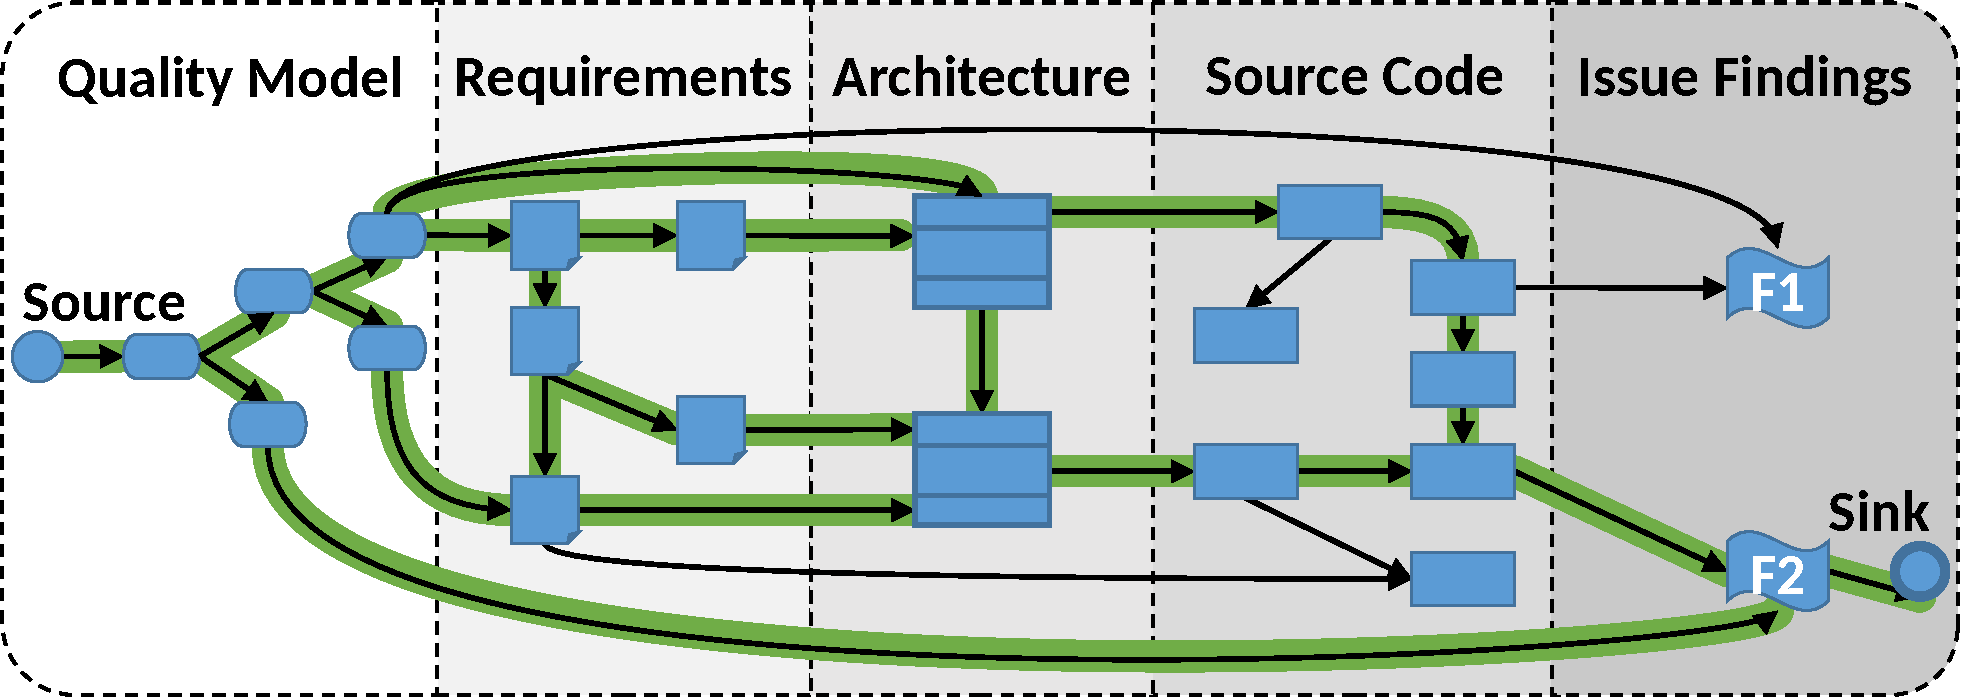
\includegraphics[width=.7\columnwidth]{figures/traces04-KG}%width=0.8\textwidth
	\caption{Example Flow Network with Typical Development Artifacts and Highlighted Flow for Issue F2}%Analysis
	\label{fig:traces}
\end{figure}

    \textbf{Aspect 1: Location of the issue.} The subsequent artifacts, such as requirements or design models, contain further knowledge about relations that \appr{} leverages for prioritization.
	For example, in practice issues may be identified in locations in the implementation that are differently connected to the rest of the code.
	Features such as logging are crosscutting and easily touch many parts of the implementation.
	Therefore, only considering flow within the implementation would over prioritize such issues.
	However, such features are only contained in planning artifacts such as design model if they are important for the project.
	By including such artifacts in the flow network, we can effectively prioritize issues.
	For example, not all nodes representing the source code in \autoref{fig:traces} are immediately connected with the requirements or design, therefore preventing direct flows towards them, lowering the total number of flow tokens that can reach issues detected on them.

    \looseness=-1
	\textbf{Aspect 2: Manual considerations.} In addition, trace links explicitly defined by security engineers or other stakeholders indicate a particular importance of the elements that are connected for the project.
	Accordingly, this could indicate that issues touching one of these elements are of higher importance.
	For example, consider an security engineer performing threat modeling on the architecture and reasoning about which threat categories, i.e., the ones of STRIDE\,\cite{STRIDE,Shostack2008}, might apply to specific elements in the architecture.
	If a possible threat is identified, this is documented whereby the threat categories considered are usually part of the quality model and it is documented to which design element this threat might apply.
	In the end, this results in a direct trace link from the quality model to the system model used at threat modeling, such as the link on top of \autoref{fig:traces} between the quality model and the architecture.
	Since these trace links lead to more edges in the flow network, it is possible to immediately propagate more flow tokens between them, therefore most likely increasing the number of flow tokens that reach an issue touching these elements, i.e., its priority.

	\textbf{Aspect 3: Security impact.} Lastly, analyzer detection rules usually indicate which quality aspects can be negatively affected by an issue detected by a particular rule, e.g., by relating the rule to common weaknesses from the CWE or listing aspects such as availability.
	These information is also embedded into the flow network and therefore considered in the prioritization.
	For example, in \autoref{fig:traces} as well F1 as F2 are immediately connected to nodes from the quality model.
%In this section, we show
%
%\begin{enumerate}
%    \item how software development artifacts connected by trace links can be converted into a flow network,
%    \item how the edges of this flow network can be weighted based on the importance of relations within the development artifacts and the relevance of the single trace links, and
%    \item how the importance of an issue can be quantified by solving the maximum flow problem for the issue.
%\end{enumerate}
%
Since prioritization using a maximum flow algorithm is straightforward after flow network construction, we focus on flow network construction.
First, in \autoref{DevArt}, we discuss which software development artifacts and trace links can be considered when constructing a flow network.
Except for a quality model, we do not give a fixed list of artifacts that must be considered, or those that are only supported by \appr{}, but discuss possible categories of artifacts, each with a concrete example using the Electronics Health Records system \emph{iTrust}\,\cite{iTrust} as running example.
For the quality model required by \appr{}, we discuss lightweight ways to obtain one.
We then show how such artifacts can be transformed into a flow network in \autoref{sec:flownetwork}.
Finally, in \autoref{sec:dsl}, we discuss in detail how arbitrary artifacts can be supported and their characteristics important for proper prioritization, such as the different types of relationships discussed above, can be reflected as weights of the edges in the flow network.
%\end{enumerate}

\subsection{Development Artifacts and Assumptions}
\label{DevArt}
%
\appr{} exploits trace links among various development artifacts that are usually created during the development of security-critical systems.
Within this paper, we assume traceability to be given such as required by many standards, e.g., the ISO/IEC 62304 for medical device software\,\cite{IEC62304}.
Existing work already investigates how to create and maintain trace links (for some approaches, see \autoref{sec:background:tracelinks}).

While conceptually \appr{} can be used with many different types of artifacts, here we describe those that we consider in the evaluation of our approach due to pragmatic reasons: Besides a quality model, they are already available for many software systems, as they are required by standards such as the ISO/IEC 62304\,\cite{IEC62304}.
Except for a quality model, they serve only as illustrative examples and developers are free to use other types of models, programming languages, or analyzers.
We describe them in the context of a running example, the \emph{iTrust} Electronics Health Records system \cite{heckman2018}.
The system has been developed as a class project at the North Carolina State University using Java and Java Server Pages~(JSP) and is repeatedly used in traceability and requirements engineering research\,\cite{zogaan2017datasets,MOHA2010,BSGRJS2018,Peldszus2019SDF,PBKJ2021,TPS2022}.


\subsubsection{Quality Model}

\begin{figure}
	\centering
	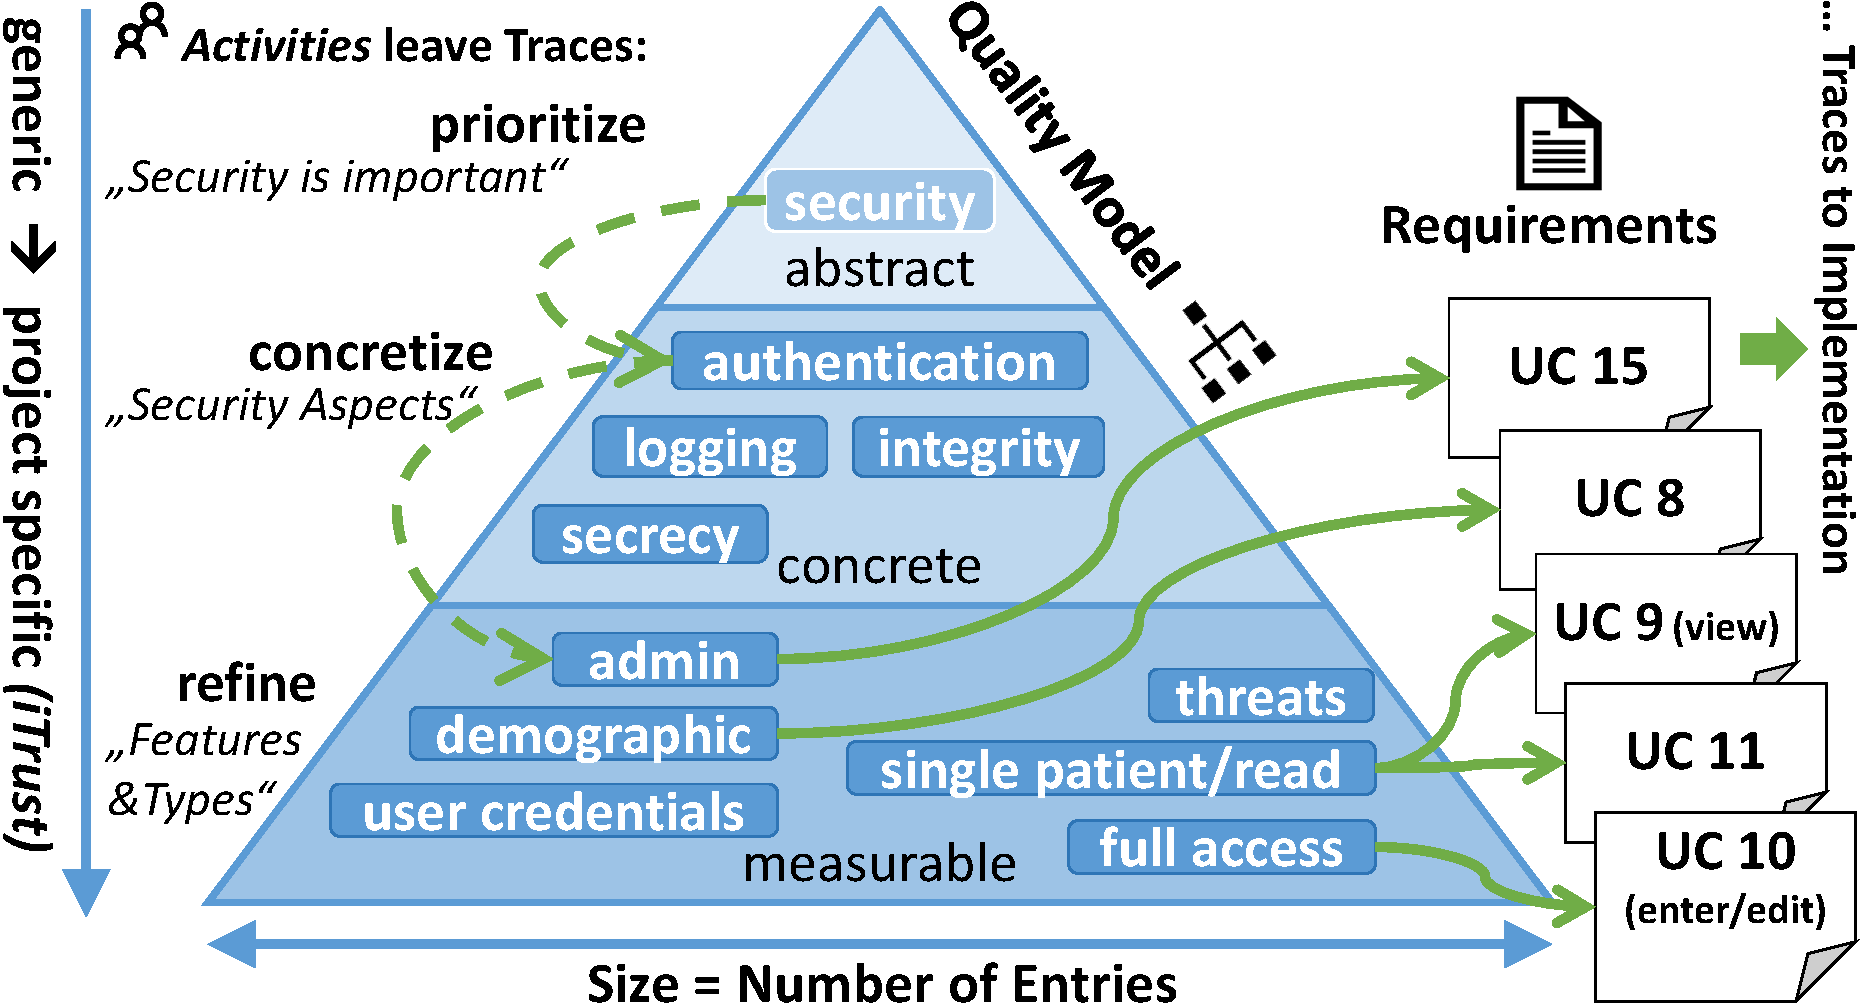
\includegraphics[width=0.7\columnwidth]{figures/QM}%0.8\textwidth
	\caption{%Refining
	Security Priorities in iTrust's Quality Model}
	\label{fig:qmodel}
\end{figure}

% Was ist ein QM?
A quality model captures, documents, and prioritizes quality aspects considered relevant for a particular project.
It is established by selecting important general quality aspects and refining them to concrete security features\,\cite{wagner2009security}.
Therefore, quality models exceed the abstract quality goals from ISO\,25010\,\cite{ISO25010,Schneider2012ASQ,WAGNER2015101}.

% Wie erstellt man ein QM im Kontext von TraceSec?
When establishing a quality model, stakeholders discuss and identify concrete, project-specific quality aspects. First, they prioritize generic qualities on an abstract level.
Next, the qualities are \emph{concretized} to relevant aspects of that quality.
This is crucial since it is an expression of a selection decision and a prioritization, which are considered indicators for relevance in \appr.
In the \emph{refinement} step, they refine types of features, affected data, or threats.
Finally, since different qualities are often seen to be of different importance to the project\,\cite{Wagner2012}, the stakeholders prioritize all quality aspects.
In particular, these different priorities of qualities need to be considered when later prioritizing issues in terms of their impact on the security of a project, since different vulnerabilities are likely to threaten different qualities.

	A quality model is the only required artifact in \appr{}.
	By considering a quality model as the reference according to which issues will be prioritized, we can capture arbitrary security aspects, such as confidentiality, integrity, privacy, or availability.
	Any relevant aspect can be captured in the quality model and will be considered in the issue prioritization.
	Thereby, different priorities of quality aspects will also be considered.

Since we consider the prioritization of security-related qualities in the quality model as the reference for relevance, \appr{} requires trace links between the quality model and subsequent artifacts, such as requirements (see \autoref{fig:qmodel}).
All downstream requirements, models, and implementations inherit their relevance from the quality model along the trace links.
While stakeholder priorities are discussed and documented in the quality model, trace links are created as a by-product of development activities.



% Wie sieht das im Running Example aus?
\autoref{fig:qmodel} shows a quality model excerpt for iTrust. %our running example.
%Since iTrust as a
Since the health application is built around the quality aspect of \emph{trust}, we assume security as quality to be of high priority.
Therefore, \emph{security} is selected at the most abstract level in \autoref{fig:qmodel}.
To demonstrate \appr{}, we look at security only, although usability or other quality aspects could be treated equally.
This is, however, beyond the scope of this paper. % which is purely focused on security issues.
In the concretization step, we identified security-related aspects of \emph{authentication}, \emph{logging}, \emph{secrecy}, and \emph{integrity} and created links to the quality aspect \emph{security}.
In the refinement step, we identified measurable units.
For example, access to purely \emph{administrative data} is considered less security-relevant than \emph{single-patient data}.
Trace links are then used to connect each quality to relevant elements from other development artifacts, such as related requirements in \autoref{fig:qmodel}.

% A quality model captures, documents, and prioritizes quality aspects considered relevant for a particular project.
% It is established by selecting important quality aspects and refining them to concrete features or non-functional requirements.
% \edit{Therefore quality models exceed} the abstract set of quality goals %requirements
% from ISO~25~010\,\cite{ISO25010,Schneider2012ASQ,WAGNER2015101}.
% %For example,
% %E.g., \emph{functional suitability}, \emph{usability}, \emph{performance efficiency}, \emph{portability}, \emph{compatibility}, \emph{reliability}, \emph{maintainability}, and \emph{security} are the top-level quality aspects in ISO~25~010\,\cite{ISO25010}. Stakeholders can use this abstract %quality
% %model %in ISO~25~010
% %to prioritize quality aspects for a given %software
% %project.

% \edit{\autoref{fig:qmodel} shows an excerpt of a quality model for our running example.}
% %\edit{For example,
% Since iTrust as a health application is built around the quality aspect of \emph{trust}, we assume security \edit{as quality} to be of high priority. %in the iTrust project,
% %if such a quality model would have been created %in the iTrust project.
% %for it.
% To this end, \emph{security} is selected on the most abstract level in \autoref{fig:qmodel}.
% To demonstrate \appr, we %will
% look at security only, although usability or other quality aspects could be treated
% equally. %accordingly.
% This analogy, however, is beyond the scope of this paper which is purely focused on security~issues.

% When establishing a quality model, stakeholders %and requirements engineers %would
% discuss and identify concrete\edit{, project-specific aspects of security, that they consider of particular importance.}
% In our running example (\autoref{fig:qmodel}), these include \edit{the security-related aspects of} \emph{authentication}, \emph{logging}, \emph{secrecy}, and \emph{integrity}.
% It is crucial to trace the refinement process \edit{since it is an expression of a selection decision and a prioritization, that are considered as indicators for relevance in \appr}.
% %We follow these choices as indicators of relevance.
% %There are several possible ways of tracing this refinement.
% \textcolor{red}{\todo{remove?}For example, one can create trace links from a refined aspect to all refining security aspects%after the refinement session
% , which can be done manually or supported by a tool.} %from security in general down to sub-aspects of security.
% In the next refinement step, \edit{and trace again)} %the
% types of features, affected data, or %potential
% threats.
% \edit{In the end, the stakeholder prioritize all quality aspects.
% We consider them the reference for relevance.}
% For example, access to purely \emph{administrative data} is considered less security-relevant %~(1)
% than \emph{single-patient data} access%~(4)
% %, or even \emph{full access} to all patient records%~(5)
% .

% %Concrete use cases or features may fall into one of those classes of security-relatedness.
% %Issues referring to high-score features will be considered more important than features that have nothing to do with security.
% \edit{\appr{} requires trace links between the quality model and requirements (see \autoref{fig:qmodel})}.
% %In \autoref{fig:qmodel}, %use cases and requirements are traced to relevant qualities\edit{, which can} occur during development, or %as a result of through reviews, %ing use cases later, as we did for iTrust.
% %In this paper, we assume those traces have been established in one way or another. %One can use traditional ways of tracing; we are also investigating techniques to facilitate creating traces. This aspect is discussed elsewhere.
% %
% %Fine-grained decisions along the process of creating the quality model lead to requirements. We consider these decisions and rationale  parts of the quality model. Requirements and use cases derived from those decisions are considered separate artifacts.
% %
% All downstream requirements, models, and implementations inherit their %importance and
% relevance from the quality model %---%and
% along the \edit{trace links}.
% \edit{
%     While stakeholder priorities are discussed and documented in the quality model, trace links are created as a by-product of those development activities. %The sequence of activities (i.e., reading a UML model, then writing a piece of code) can be traced manually, through commit messages, or in a dedicated editor.
% }
% %We map the propagation of importance from a quality model to implementations and warnings or issues to the maximum-flow model depicted in \autoref{fig:traces}. Importance flows along the traces from quality priorities %(in the quality model)
% %to requirements closely related to those high-priority quality aspects, down to model and code implementing those same requirements.

\subsubsection{Requirements}



As requirements are documented in various forms, from textual to formal models, to effectively exploit traceability information, it is recommendable to use a model focused on their trace links %, which abstract
and abstracts
from the actual notation.
For this, we use in our example a simplified adaption of \emph{T-Reqs}\,\cite{Grosser2022RDR}, that represents requirements and flows in a model-based fashion.
This allows us to reference requirements and their flows with trace links.

In the running example iTrust, the requirements are specified in 79 use cases, 36 of which are implemented in version 21 of iTrust.
Each use case is documented textually on an individual wiki page\,\cite{iTrustWiki}.
E.g., use case UC26 (see \autoref{fig:uc26}) describes the management of laboratory procedures by Health Care Personnel (HCP).
%\figurename~\ref{fig:uc26}  shows an excerpt of the model, we derived
We automatically derived a requirement model
%from this %textual representation
to obtain individual requirement objects and relations. % among them. %which can be used for our approach.
%The requirement metamodel with set-containment and typed relations is a simplified adaption of the \emph{T-Reqs} model\,\cite{Grosser2022RDR}.
For this, we extracted containment relations from the given section structure and additional trace information from hyperlinks and text labels, as illustrated in \autoref{fig:uc26}.
%
%\begin{figure*}
%	\centering
%	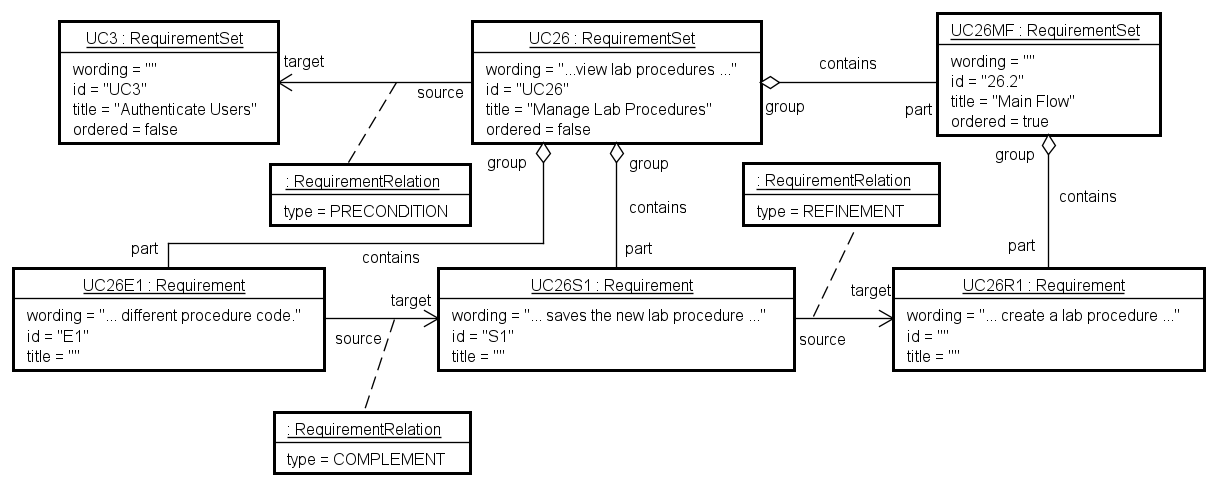
\includegraphics[width=0.8\textwidth]{figures/UC26_Objectdiagramm_wide.png}
%	\caption{Excerpt of Requiremets Model for iTrust UC26}
%	\label{fig:uc26}
%\end{figure*}
%
For example, UC26 contains the pre\-condition that requires the users to authenticate themselves (linking to use case UC3).
%The
A main flow section, consists of individual requirements, describes the general sequence of actions, %. %\autoref{fig:uc26} shows the main flow with its first requirement, describing lab procedure creation. As most main-flow requirements, it is
%This can be
and is refined by more detailed sub-flows. %, the requirement with ID \enquote{S1}.
Alternative flows describe actions with complementary conditions, e.g., deficient inputs. %, and are referenced from main or sub-flows. %S1 is complemented by the requirement \enquote{E1}. UC26 contains further sub and alternative flow requirements, as well as
Use cases contain additional requirements for logging events and links to other use~cases. %, not depicted in \figurename~\ref{fig:uc26}.

\begin{figure}
	\centering
	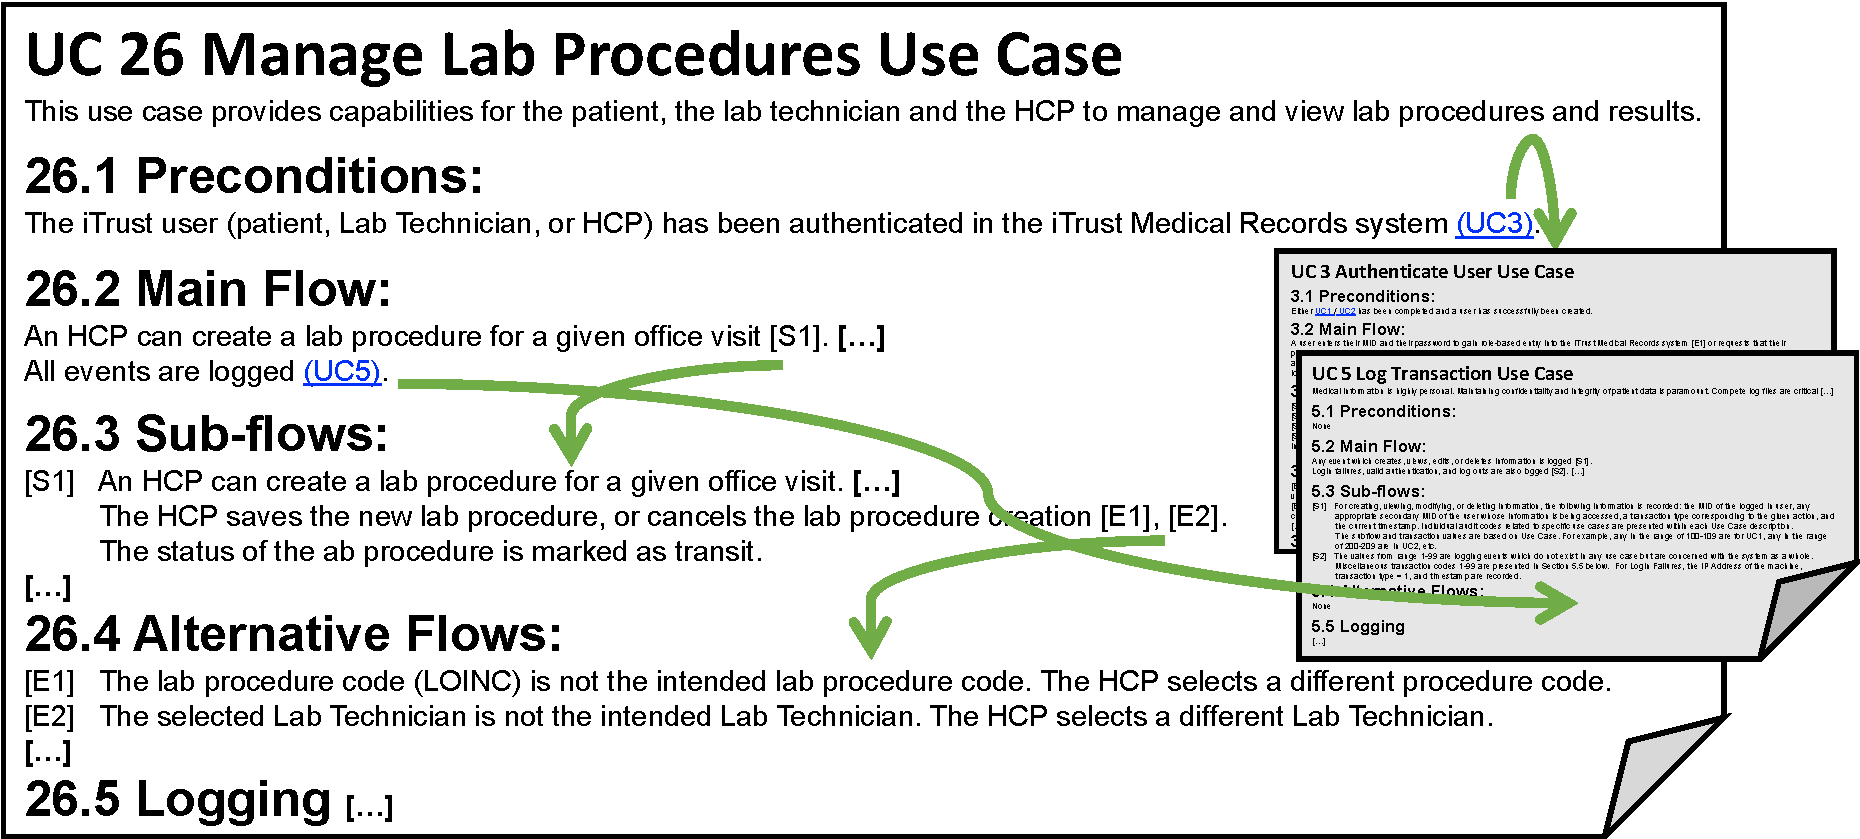
\includegraphics[width=0.9\columnwidth]{figures/UCexample2}
	\caption{Excerpt of iTrust UC26 and its dependencies; HCP = Health Care Personnel}
	\label{fig:uc26}
\end{figure}

\subsubsection{Architecture}

\begin{figure}
	\centering
	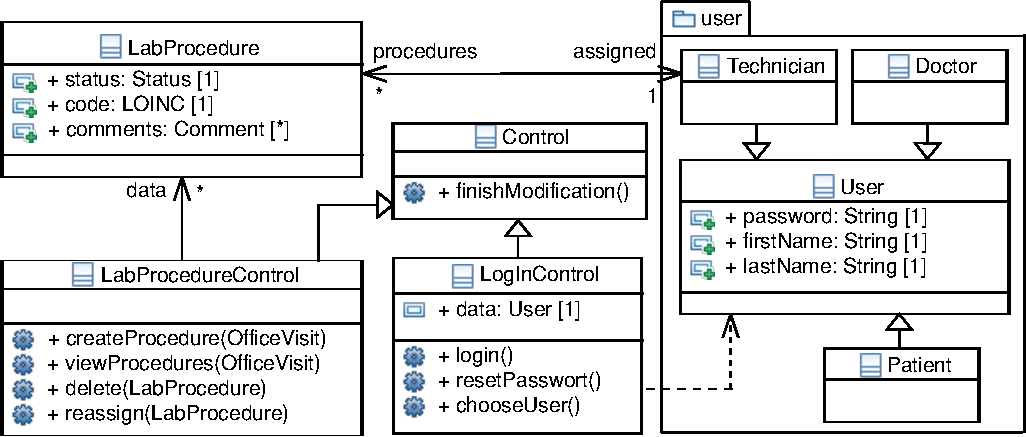
\includegraphics[width=.75\columnwidth]{figures/itrust-classdiagram-labprocedure.pdf}%0.8\textwidth
	\caption{Excerpt from the iTrust Class Architecture}% of the iTrust System
	\label{fig:clsarch}
\end{figure}

At systems development, architecture specifications should express the fundamental relationships among architectural elements and are a mean for planning and documenting the system implementation\,\cite{CGL+03}.
In \appr{} we support model-based rep\-resentation of the major structural elements and their interrelations as architecture specification, e.g., component-and-connector views\,\cite{Ivers2004DCC,Bertram2017}.
If architectural models are used, we need the architectural structures to relate structural elements to the requirements and the quality model.
In this way, we specify which structural elements are particularly relevant for the quality goals.

While \appr{} allows for any or even multiple architecture description languages, in the running example, we use an architecture specification utilizing the Unified Modeling Language (UML),
a widespread standard for specifying software architectures\,\cite{uml}.
In various works, UML models specifying the architecture of iTrust have been reverse-engineered\,\cite{MOHA2010,BSGRJS2018,PBKJ2021}.
%In this work, we are using these as architecture specifications in our evaluation. %as well as for the introduction of the iTrust system’s architecture.
%
The requirements of iTrust are realized by \emph{Control} classes for each use case, complemented by classes for data.

\autoref{fig:clsarch} shows an excerpt from the class architecture showing these controls and classes representing users of the system:
%
The class \textit{LaboratoryProcedureControl} realizes the management of laboratory procedures as specified in UC26, while \textit{LoginControl} realizes the required authentication as described in UC3. For all classes, essential data and functionality is specified as properties and operations. %These are going to be detailed and realized in the implementation.

	In practice, the design may not map as conveniently to the requirements.
	Nevertheless, the software architects usually develop a system design having the requirements at hand, thereby manually recording trace links.
	In the end, providing at least some traceability is unavoidable, since developers are assigned tasks to implement specific requirements at a given location in the system design.
	This information is usually provided more or less explicitly, e.g., via ticket systems.
	If not provided, developers have to manually search for the corresponding locations in the system and should document this information.
	As briefly discussed in \autoref{sec:background:tracelinks}, there also exist approaches for automated trace link retrieval between requirements and architecture\,\cite{Goknil2014,Keim2024}.

\subsubsection{Threat modeling}
Threat modeling is a technique to systematically identify possible threats to the system under development\,\cite{Shostack2008}.
In popular threat modeling approaches such as STRIDE\,\cite{STRIDE,Shostack2008} or PASTA\,\cite{pasta}, the system is represented at a coarse-grained level to allow systematic reasoning about possible threats to the system.
A common representation used for this purpose is data flow diagrams, but any abstract system model could be used, e.g., UML models defining an abstract system design.

Based on these diagrams, security experts reason about possible threats for each element in the diagram. Frameworks such as STRIDE assist the experts by providing types of threats that can compromise the security of a system. STRIDE itself is an acronym that stands for the categories that need to be considered: Spoofing, Tampering, Repudiation, Information Disclosure, Denial of Service, and Elevation of Privilege.

Ultimately, these types of threats comprise qualities that are expressed in the quality model, i.e., an instance of the threat of spoofing would threaten the quality ``authenticity'' shown in \autoref{fig:qmodel}.
The considered threat types are documented in the quality model as qualities, possibly accompanied by custom project-specific qualities.
When security experts reason about and document threats in the system representations, this information can be used as trace links from the quality model to the design models inspected during threat modeling.
	Each identified threat results in an explicit trace link between the threatened design element and the threat, i.e., quality from the quality model.
	For example, the direct edge between the quality model and the architecture in \autoref{fig:traces} results from such a trace link.

In the case of limited resources, only the qualities of the selected threat model can be considered to manifest a quality model.
For STRIDE, the quality model would merely consist out of the six threat categories, which could be ranked according to project needs or be considered as equally important.

In addition to STRIDE, there are several other threat modeling frameworks that provide different types of threats that can be considered.
For example, LINDDUN\,\cite{deng2011privacy} provides threats tailored to privacy. When several of these frameworks are used, the quality model serves as a means to relate them.

\subsubsection{Source Code}
\appr{} needs the program code as a processable model at an appropriate level of abstraction.
We need knowledge about containment relationships (e.g., classes in a package, methods in a class) as well as cross-references (which method calls which other method).
Various tooling, such as MoDisco \cite{modisco} or JaMoPP \cite{jamopp}, exists to extract such models from source code written in specific programming languages, i.e., Java.
However, while these tools resolve references such as method calls, these usually contain all details from the statement level, leading to huge models.
We use the GRaViTY program model\,\cite{PKLS2015,Peldszus2022,Peldszus2024} for making this information accessible.
%For the analysis of the system’s source code, we use the GRaViTY program model\,\cite{PKLS2015,Peldszus2022}.
The program model provides an abstraction from the fine-grained abstract syntax tree reducing details from the statement level of methods and fields to explicit dependencies between these, e.g., calls between class members.
This abstraction allows considering fewer details %on the statement level
of the implementation, i.e., 28\% fewer nodes than a MoDisco model \cite{Peldszus2024}, when prioritizing issues, which reduces the size of the flow network and improves the run-time overhead.
Finally, the GRaViTY model is designed to support arbitrary object-oriented programming languages \cite{PKLS2015}, therefore providing the flexibility to support further programming languages besides Java.

\autoref{fig:javaiTrust} shows an excerpt of the program model extracted from the running example's source code focusing on the edit of a lab procedure implementing the class \textit{LaboratoryProcedureControl} from the class design in \autoref{fig:clsarch}.
The excerpt focuses on the addition of a comment to a laboratory procedure through a \textit{LabProcedureForm}, which is one of the classes realizing the \textit{LabProcedure} from the class design, using its method \textit{addCommentary}.
Adding a comment includes various calls to other functionality such as \textit{edit} to update the status that is stored in the field \textit{labProcedureStatus}.

\begin{figure}
	\centering
	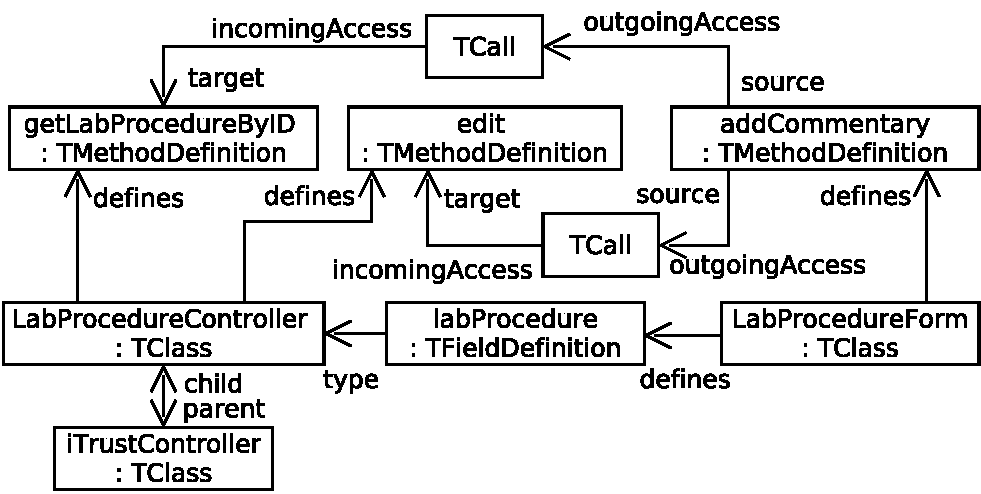
\includegraphics[width=.65\columnwidth]{figures/java-itrust-editLabProcedure}%0.8\textwidth
	\caption{Excerpt from the iTrust Program Model}
	%\caption{Excerpt from the Program Model of the iTrust System showing the Edit of a Lab Procedure}
	\label{fig:javaiTrust}
\end{figure}

\subsubsection{Issues}
Many analyzers, such  as SonarQube\,\cite{sonar}, SpotBugs\,\cite{SpotBugs}, PMD\,\cite{pmd}, CodeQL\,\cite{codeql}, and many others, analyze source code for implementation issues.
To do this, these analyzers typically rely on detection rules that express known violation patterns.
These weaknesses expressed in the rules can usually be immediately related to qualities from the quality model.
Since all of these analyzers detect concrete vulnerable code statements, we assume that issues in \appr{} are always related to concrete code locations, and optionally have further relationships to quality aspects that are threatened by the type of issue.

\looseness=-1
In this work, we compute issues with SonarQube, but any other static analysis tool will work.
Therefore, the following describes how to integrate an analyzer into \appr{}, using SonarQube as an example.
Just as the elements from all other models, issues detected by SonarQube must be connected with all relevant elements, i.e., the code location at which the issue has been detected or affected qualities in the quality model, via trace links.
To realize the necessary trace links to the source code, we use an extension mechanism of GRaViTY\,\cite{peldszus2016continuous} and annotate program model elements with the issues. To navigate to the lines of code where the issues are located, we keep a reference to the file and line.
%to add them directly as annotations.
Furthermore, SonarQube’s detection rules can contain references to relevant security aspects, e.g., when the issue targets a concrete weakness, e.g., one of these captured in the common weakness enumeration (CWE)\,\cite{cwe}, further underlining their importance.
%For example,
In the running example, the two issues in \autoref{fig:traces} are vulnerabilities directly threatening a security aspect in the quality model. Nevertheless, based on their location in the code, they do not have the same priority.

\subsection{Converting Artifacts into a Flow Network}
\label{sec:flownetwork}
%
%The first problem we have to solve if we want to calculate the maximum possible flow through a network from a source to a number of sinks is the creation of this network.
%In our case, the sinks are the findings of static analyzers, the network is given by the trace links and dependencies within the development artifacts, and the source is the root of the quality model.
%In what follows, we describe in detail how to create a flow network from the development artifacts of a software project and trace links between these.
%
%Traces indicate references to previously developed elements and therefore build the connection between the different artifacts.
To create a flow network (step 2 in \autoref{fig:PrioApproach}), we assume that every trace link can contribute to the importance of an element and
thus
is %therefore
represented by an edge in the flow network. As we %are going to
propagate importance from the quality model to the findings, we assume every edge derived from a trace link to point in this direction. All elements connected by trace links become nodes of our flow~network.

Nodes added to the flow network based on trace links may also be interconnected via relations within the development artifacts.
%The nodes added to the flow network based on the trace links may also be connected through relations within the single development artifacts.
For example, two classes linked by trace links may be in an inheritance relationship.
Such relations also contribute to the flow network as edges.
The new element and its relations are added to the flow network recursively to include all potentially relevant elements and relations.
Finally, we get an iterative construction algorithm that terminates when there are no more relations to~process.

\begin{algorithm}
        \caption{Flow Network Creation}
        \label{algo}
		\SetKwInOut{Input}{Input}
		\SetKwInOut{Output}{Output}

		\Input{Set of Trace Links \emph{traces}, Quality Model \emph{qm}}
		\Output{Flow Network G(\emph{nodes}, \emph{flows})}
		\BlankLine
		stack := \{qm$\rightarrow$allRelations()\}\;
		flows := \{\}\;
		nodes := \{node(qm)\}\;
		\BlankLine

		\ForEach{t $\in$ traces}{
			src := nodes$\rightarrow$getOrCreate(t.src)\;
			trg := nodes$\rightarrow$getOrCreate(t.trg)\;
			flows$\rightarrow$add(src, trg, capacity(src, trg))\;
			stack$\rightarrow$addAll(t.src$\rightarrow$allRelations())\;
			stack$\rightarrow$addAll(t.trg$\rightarrow$allRelations())\;
		}
		\BlankLine
		seen := \{\}\;
		\While{stack$\rightarrow$hasNext()}{
			relation := stack$\rightarrow$pop()\;
			\BlankLine
			\If{!seen$\rightarrow$contains(relation) \&\& consider(relation)}{
				seen$\rightarrow$add(realtion)\;
				src := nodes$\rightarrow$getOrCreate(relation.src)\;
				trg := nodes$\rightarrow$getOrCreate(relation.trg)\;
				flows$\rightarrow$add(src, trg, capacity(src, trg))\;
				stack$\rightarrow$addAll(relation.trg$\rightarrow$allRelations())\;
			}
		}
\end{algorithm}

\autoref{algo} shows how the flow network can be created, considering trace links and the relations within single artifacts.
The algorithm takes a set of trace links among the development artifacts and a quality model as input.
%a quality model and all trace links among the development artifacts and returns a flow network.
In lines 1--3, data structures for building the network are initialized.
These comprise sets of all nodes and all flows in the constructed flow network and a \texttt{stack} for storing relations among development artifact elements that have to be processed.
To guarantee that the entire quality model will be added to the flow network, the set of \texttt{nodes} is initialized with a node representing the root of the quality model, and the stack of unprocessed references is initialized with all outgoing references.
First, we iterate over all trace links in lines 4--10 and add flows expressing each trace link to the flow network.
In lines 5--6, we retrieve the nodes corresponding to the trace link's source and target or create corresponding nodes if the element has not been processed yet, using a helper function \texttt{getOrCreate}.
Afterward, we add an edge between these two nodes to the flow network (line~7).
Here, we also calculate the edge's capacity (see \autoref{edgeCap}).
In lines 8--9, we add all outgoing relations of the trace link's source and target to the stack of unprocessed relations for being processed after all trace links have been processed.

After leaving the loop in line 4, all trace links are represented by edges in the flow network but the connections within the different artifacts are missing.
Starting from line~11, we add these additional elements to the flow network.
To avoid adding edges twice, we first initialize a stack containing all relations that have been processed (\texttt{seen}).
Afterward, in lines 12--21, we process all  references that have been put on the reference \texttt{stack}.
According to  line 14, we add a reference to the flow network if it has not been added before (not being on the \texttt{seen} stack) and the relation is not ignored by the user (see \autoref{edgeCap}).
For determining if a relation is not ignored and therefore should be considered, we use a helper function \texttt{consider} that will be explained afterward.
If a relation is to be added, we first put it on the stack of seen references and proceed as we did for the trace links.
As the target of the reference might contain references that have not been considered yet, we add all outgoing references to the relation stack.
Once the relation stack is empty, the flow network has been constructed successfully.

At network construction, we want to only consider the relation types that contribute to propagating importance.
%As not every kind of relation contributes to propagating importance, we only consider the kinds of relations that can do so.
This filtering allows us to create flow networks faster and reduces the effort of solving the maximum flow problem as the flow network will be smaller.
%In the next section,
Next, we introduce how this filtering can be tailored towards concrete projects and how edge capacities will be determined.

\subsection{Filtering and Determining Edge Capacities}\label{edgeCap}
\label{sec:dsl}
%
\noindent
In \appr{}, we aim to support arbitrary artifacts created during development.
Besides those considered in our example, common artifacts include data flow diagrams (DFD) for threat modeling\,\cite{Shostack2008,TUMA2018275}, business process models (BPMN)\,\cite{white2008bpmn}, Palladio component models\,\cite{reussner2011palladio}, other, perhaps even security-specific, requirements models\,\cite{8004340}, and many others.
For each of these model types, it is necessary to specify how to integrate them into a flow network.
Furthermore, it may even be project-specific which elements to consider and how to consider them.
For this reason, it is not possible to integrate this logic directly into the network construction.
To this end, we allow an exchangeable and reusable artifact import specification of what should be considered when constructing the flow network, allowing even project-specific considerations to be taken into account.
To achieve this, we have specified a domain-specific language (DSL)\,\cite{fowler2010domain,dsl} that allows specifying not only which reference types should be included, but also which capacities should be assigned to the corresponding edges in the flow network.
This DSL allows experts, such as maintainers of a particular modeling language, to specify artifact import specifications to support specific artifacts in prioritization.
Other security experts of companies using \appr{} can take these specifications and optimize them according to project characteristics, e.g., to optimize the created flow network by considering the level of detail in design models, the amount of available trace links, or to define metamodels for specific model types used in the project.
Afterwards, the prioritization can be performed by all developers without taking these details into account, just by using the provided configurations.
Our examples provide default settings for common artifact types.

Since the source of the maximum flow problem is the root of the quality model and the sink an issue in the implementation, we are searching for the maximum flow from the most coarse-grained element to one of the most fine-grained element.
Therefore, when adding edges to the flow network, we refine importance in the context of system refinement.
%Therefore, when adding edges to the flow network, the underlying assumption is that importance always flows \emph{from coarse-grained elements to fine-grained elements}.
If we would allow flows in the opposite direction, this would allow additional flows over entirely unrelated elements and therefore prevent proper prioritization.
For example, consider a flow from a requirement to an element in the system design that then propagates trough the design until it reaches an design element relevant to an additional unrelated requirement, which will eventually happen in every system unless it could be split into two independent systems.
This second requirements then has relations to additional parts of the implementation entirely unrelated to the first requirements but will allow flows that suggest an relation.
To this end, it is not necessary to explicitly specify the direction in which trace links should point or whether they should be considered, but only the order of the artifacts between which trace links exist.
In the construction algorithm, all trace links are added to the flow network and the direction is derived from the order of the artifacts.
It is also necessary to calculate the capacity with which they should be added.
For example, a direct trace from the quality model to the implementation is more important than a trace to the architecture, which should be reflected in the capacities.
In our approach, the capacity of edges representing trace links depends on the distance between the models, with the desired order specified by the user.
In our example, we assume the following order of artifacts (as in \autoref{fig:traces}):

\begin{small}
\begin{description}
\item \texttt{Quality Model (0) < Requirements (1) < Archi\-tec\-ture~(2) < Program Model~(3) < Findings~(4)}.
\end{description}
\end{small}

%Weights (represented as capacities in the flow network) express how heavily the different coarse-grained security aspects in the quality model are affected by a detected issue.
However, there is no explicit capacity assigned to each individual trace link---neither in a project nor in our approach.
%In this paper, we postulate the existence of those traces, no matter how they were created. Creating traces as a by-product of project activities is a separate line of work we conduct in parallel. It is beyond the scope of this paper.
We assume that every \emph{stage} is assigned with an increasing value allocated to the nodes representing entities from these development artifacts.
The concrete capacity of a flow edge representing a trace link is calculated by a customizable function \texttt{capacity(Node, Node)}, calculating the capacity based on the distance between the nodes.
For simplicity, we show a linear function that only adds a static configuration factor for adjustment, e.g., selected depending on how intensively trace links are created within a project:

\begin{small}
\begin{description}
\item
\texttt{capacity(Node a, Node b): abs(a.stage-b.stage) $\times$ factor}.
\end{description}
\end{small}

In addition to direct trace links between elements of individual artifacts, there are also indirect trace links, such as through inheritance or containment relationships within an artifact.
To this end, besides trace links, we have to consider different edge types from the models: % in our flow network:
%First, there are edges whose capacity can be determined based on their type, e.g., inheritance or refinement links.
%Second, there are also edges whose capacity should be determined based on the concrete model instance:

\begin{enumerate}[label=\alph*)]
    \item To allow the customization of quality relevance, in the quality model custom priorities can be specified.
    These priorities should be reflected as capacities of the flow edges pointing to the nodes representing a quality.
    \item In all other models, the capacities are not specified individually %based on the concrete instances
    for each instance but the considered relationship types are associated with capacities.
    %These capacities can be statically specified using a configuration file.
    E.g., one can assume that every flow edge created for a \textit{Generalization} will have the capacity 1 and every \textit{Containment} %relation
    the capacity~2.
\end{enumerate}

How to handle these edges is specified in the proposed DSL.
While \autoref{lst:grammar} provides the syntax of the DSL, \autoref{dsl} shows an instance that contains exemplary specifications that make the metamodels of three artifact types used in the running example of this work accessible to \appr{}.
By using additional instances or by extending the shown one, arbitrary metamodels can be made accessible to \appr{}.
We explain the syntax of the DSL on the example.
The syntax itself is written in the Xtext\,\cite{xtext} language grammar, which is similar to the Extended Backus–Naur Form (EBNF)\,\cite{Yue2014}.

Each instance represents a \texttt{Configuration} that makes an arbitrary number of metamodels, e.g., for representing requirements or design models, accessible to \appr{}.
We assume that the metamodels are organized by \texttt{Namespace}s, as in the Eclipse Modeling Framework (EMF)\,\cite{steinberg2008emf, EMFBook}.
For each namespace, one can specify a default capacity for all references within the metamodel and whether all its elements should be considered by default or not.

For example, in lines 1--4 of \autoref{dsl}, in the artifact import specification for the UML metamodel, we specify that all elements should be included with a capacity of~2.
This is the simplest case needed to support an artifact type, i.e., all elements specified in its metamodel, in \appr{}.
These artifact import specifications may become more complicated, as our UML specification does, to reflect the characteristics of the modeling languages.
We will demonstrate this with the other two artifact import specifications shown in \autoref{dsl}.

For the GRaViTY program model, in lines 6--15, we include also all elements by default, but additionally, specify special handling of two elements.
For every namespace, one can specify which of the types that are defined in the metamodel should be included or excluded when building the flow network.
Again, in the grammar rule \texttt{Type}, the same default values as for namespaces could also be defined on the scope of single types.
Within a type, one can specify references that should be included or excluded.

\lstset{
    string=[d]{"},
    stringstyle=\color{blue}
}
\begin{lstlisting}[caption={Grammar of the DSL structured into multiple grammar rules}, label=lst:grammar, float, keywords={enum,INT,STRING},basicstyle=\small\ttfamily,breaklines]
Configuration:
  ("default" "=" default=INT)?
  ("consider" "=" consider=Consider)?
  (namespaces+=Namespace)+;

Namespace:
  "namespace" package=STRING "{"
    ("default" "=" default=INT)?
    ("consider" "=" consider=Consider)?
    ("include" "{" (include+=Type)* "}")?
    ("exclude" "{" (exclude+=[ecore::EClass])+ "}")?
  "}";

Type:
  "type" type=[ecore::EClass] "{"
    ("consider" "=" consider=Consider)?
    ("default" "=" default=INT)?
    ("include" "{" (inlcude+=Edge)+ "}")?
    ("exclude" "{" (exclude+=[ecore::EReference])+ "}")?
  "}";

Edge:
  "reference" reference=[ecore::EReference] ("--" type=[ecore::EClass]
    ("--" target=[ecore::EReference])?
  )? direction=Direction weight=Weight;

Weight: NumberWeight | AttributeWeight;
NumberWeight: value=INT;
AttributeWeight: value=[ecore::EAttribute];

enum Consider: ALL="ALL" | NONE="NONE";
enum Direction: FWD="->" | BWD="<-" | BI="<->";
\end{lstlisting}

%\vspace{-4pt}
%float,
\begin{lstlisting}[
    language=Java,
    basicstyle=\small\ttfamily,
    numbers=left,
    tabsize=1,
    breaklines=true,
    morekeywords={namespace,default,consider,include,type,reference,exclude},
    caption={Example for the use of the DSL for Specifying a Configuration for Creating the Flow Network},
    label=dsl,
    float
]
namespace "http://www.eclipse.org/uml2/5.0.0/UML" {
 default = 2
 consider = ALL
}

namespace "http://www.gravity-tool.org/typegraph/basic" {
 default = 2
 consider = ALL
 include {
  type TMember {
   include { reference accessing--TAccess--target -> 1 }
  }
 }
 exclude { type TAnnotation }
}

namespace "http://www.tracesec.org/qualitymodel" {
 consider = NONE
 include {
  type Quality {
   include { reference aspects--Aspect--quality -> priority }
  }
 }
}
\end{lstlisting}


%\begin{lstlisting}[
%    language=Java,
%    basicstyle=\footnotesize\ttfamily,
%    numbers=left,
%    tabsize=1,
%    breaklines=true,
%    morekeywords={namespace,default,consider,include,type,reference,exclude},
%    caption={Configuration for building the flow network},
%    label=dsl,
%    float
%]
%namespace "http://www.eclipse.org/uml2/5.0.0/UML" {
% default = 2
% consider = ALL
%}
%
%namespace "http://www.gravity-tool.org/typegraph/basic" {
% default = 2
% consider = ALL
% include {
  %type TMember {
%   include {
%    reference accessing--TAccess--target-> 1
%   }
%  }
% }
% exclude {
%  type TAnnotation
% }
%}
%
%namespace "http://www.tracesec.org/qualitymodel" {
% consider = NONE
% include {
%  type Quality {
%   include {
%    reference aspects--Aspect--quality-> priority
%   }
%  }
% }
%}
%\end{lstlisting}


For includes and sequences of references, we can specify the inclusion of references pointing only to certain types, and the capacity and direction of the corresponding edge in the flow network (cf. grammar rule \texttt{Edge}).
In lines 10--12, we specify how accesses between class members (\texttt{TMember}) are considered.
Instead of \texttt{TAccess} nodes, the pair of references \texttt{accessing} and \texttt{target} will be added as a single edge in the flow network.
Furthermore, the direction in which the edge will point in the flow network is specified (\texttt{->, <-, or <->}), in this case in the reading direction.
Finally, due to the usually high number of accesses in an implementation, we specify that the edges should only be considered with a capacity of 1 instead of the default value of 2, to allow a more fine-grained propagation of flow tokens.
While the purpose of this value mainly is to demonstrate the capabilities of the DSL, it still stems from an practical observation.
However, the concrete value should be determined based on long-term experiences.

%Finally, as in our example only annotations such as \textit{@Deprecated} are used, annotations have only a connection to the annotated element and cannot contribute to the flow network but will grow it unnecessarily, we exclude these in line~14.

As the last part of the artifact import specification for the GRaViTY program model, annotations are excluded in line 14.
Those used in the example implementations, such as \textit{@Deprecated}, only link to the annotated element and cannot contribute to the flow network, but will make it grow unnecessarily.
In the full specification for the program model, however, this exclusion of annotations is overridden by a more fine-grained specification that considers issue annotations, which are subtypes of \texttt{TAccess} and would otherwise also be excluded.


%\edit{We include no element from the quality model} by default but only those explicitly specified \edit{(only the nodes of type \texttt{Quality}).
%The user-defined priority of a \texttt{Quality} is defined on an \texttt{Aspect} node between the quality and its parent \texttt{Quality}.}
%As for the accesses among members, we do not add these nodes to the model.
%As the capacity of the resulting edge, we use the value stored in the attribute~\texttt{priority}.

We include only explicitly specified elements of the quality model (i.e., only the nodes of type \texttt{Quality}).
Like the accesses among members, we do not add these nodes to the model.
The user-defined priorities in the quality model, which should be considered as edge capacities, are defined in a \texttt{priority} attribute of an \texttt{Aspect} node.
This node relates two \texttt{Quality} nodes to each~other.

Using this DSL, experts can specify default values for the scope of namespaces and types.
Furthermore, specific elements can be explicitly excluded or included in the flow network construction.
Finally, for each reference type, a static capacity or a pointer to an attribute holding the capacity can be specified.
To the end user using the \appr{} issue prioritization, these specifications are black-boxes, and they use only the artifact import specifications that are provided to them by experts.
	While we show a concrete optimization based on a practical observation, we explicitly avoided detailed optimizations in this work.
	The configurations used in this work are as simple as those shown above and are still suitable to achieve proper prioritization.
	Therefore, the effort needed to support a different metamodel is as low as writing 4 lines as for the UML example shown in \autoref{dsl}.
	However, there is still an opportunity for detailed fine-tuning if needed, e.g., due to further observations similar to the one described.
%Finally, per included element a static capacity can be specified or a pointer to an attribute of the model instance.